
\chapter{Experiments and Evaluation}

\section{Lab Tests}

Parallel to building prototype RobotME Framework we were also building mobile application
that can be used to verify our framework capabilities. This application use each
kind of visual component with each possible features that the testing framework
supports.

Most of our tests were performed on emulators of real devices, usually using
generic emulator provided by Sun Microsystem called WTK (Wireless Toolkit) but also
SonyEricsson's and Nokia emulators. It was
because it is the fastest way of deploying mobile application and than executing it,
and during constant development there is simply no time for time consuming
deployment on real devices. After the prototype was created we performed several tests on 
real devices, including: SonyEricsson P900i (that supports CLDC 1.1 standard) and
SonyEricsson K610i (that on the other hand supports CLDC 1.0 standard). Our framework
supports all mobile devices that conforms to at least standards: MIDP 2.0 and
CLDC 1.0 so theoretically these two devices should be fully supported by RobotME
Framework.

Testing devices were connected to the Log Server through GPRS connection. For each of
visual component our framework supports dedicated scenarios were recorded. Then
we tried to replay previously recorded scenarios. When replaying scenario finishes
with success (no assertion was violated) then we modified scenario so that it should no longer
be correct and hoping that during next replaying process assertions will be violated
and tests will not pass. It was indeed in our case. All of tests passed when it
intended to, and all assertions was violated when we manually modified scenarios.

The example of one event that could be modified in the scenario so that whole scenario
will not pass could be as follows. It presents snapshot of states items on the form
that is currently shown on the device's screen.

Before modification:

\begin{xmlblock}
	<event level="INTERNAL" timestamp="1166970731531"
		replayable="false" assertion="true">
		<form-modification title="Form Title 1">
			<items>
				<choice-group label="Choice group label">
					<selectedFlags>
						<value>true</value>
						<value>false</value>
						<value>true</value>
					</selectedFlags>
					<strings>
						<value>Option 1</value>
						<value>Option 2</value>
						<value>Option 3</value>
					</strings>
				</choice-group>
				<date-field label="Date 1" date="1166970731529" />
				<gauge label="Gauge 1" value="6" />
				<image label="Img 1" altText="Alternative text 1" />
				<spacer />
				<string-item label="String item 1" text="Text 1" />
				<text-field label="Text field 1" string="String 1" />
			</items>
		</form-modification>
	</event>
\end{xmlblock}

After modification (form title was changed):

\begin{xmlblock}
	<event level="INTERNAL" timestamp="1166970731531"
		replayable="false" assertion="true">
		<form-modification title="Form Title 2">
			<items>
				<choice-group label="Choice group label">
					<selectedFlags>
						<value>true</value>
						<value>false</value>
						<value>true</value>
					</selectedFlags>
					<strings>
						<value>Option 1</value>
						<value>Option 2</value>
						<value>Option 3</value>
					</strings>
				</choice-group>
				<date-field label="Date 1" date="1166970731529" />
				<gauge label="Gauge 1" value="6" />
				<image label="Img 1" altText="Alternative text 1" />
				<spacer />
				<string-item label="String item 1" text="Text 1" />
				<text-field label="Text field 1" string="String 1" />
			</items>
		</form-modification>
	</event>
\end{xmlblock}

Please note that the same event XML definition could be used as an assertion
(if appropriate attributes are set to: replayable="false" assertion="true") but also
could be used to simulate user interaction with the mobile application
(if this attributes are set to: replayable="true" assertion="false").

\section{Real-life Use Case}

\begin{figure}[t]%
\begin{center}
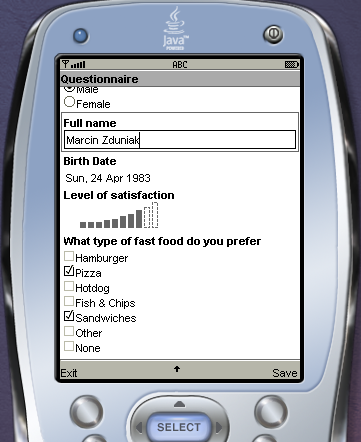
\includegraphics[width=.6\linewidth]{figures/screen-1b-emulator}
\end{center}
\caption{Emulator window with example mobile application under test.}%
\label{fig:screen-1b-emulator}
\end{figure}

\begin{figure}[t]%
\begin{center}
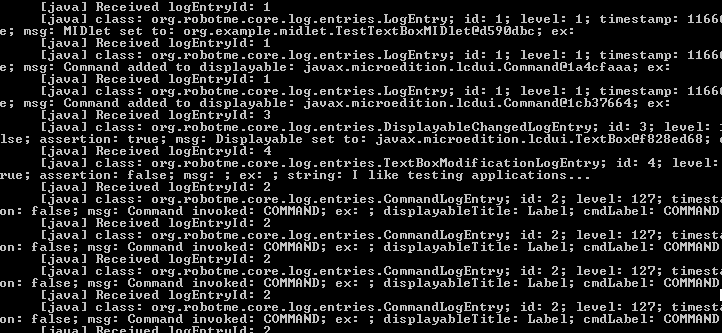
\includegraphics[width=\linewidth]{figures/screen-2-console}
\end{center}
\caption{Server console -- Log Server.}%
\label{fig:screen-2-console}
\end{figure}

As we were starting our work on this framework we were not sure if our idea is
even possible to realize and implement, there are no similar frameworks
for mobile platforms created before. We started from creating code that is
able to intercept events from the mobile phone as well as correctly
simulate them. Our prototype demonstrated it is possible.

The next thing that is still in front of us is verifying our framework against
real mobile application, that is not only a set of related screens created by
us to only demonstrate some Frameworks capabilities, but that that
have some useful logic behind this screens. Natural choice for candidate of such
application is NaviExpert, application created by group of researchers and
students from Poznan University of Technology intended to navigate simple
mobile phone users from one point to the other using back-end server and
GPS connected to the phone or embedded into mobile device. At this moment our prototype
solution is not ready to capture all important events in NaviExpert and
properly replay them. The points that must be addressed before being able to
test that application are:

\begin{itemize}
\item more kind of assertions need to be implemented, especially those related to 
  Record Store, sound events and various means of data transferring over the air like:
  bluetooth or GPRS connections.
\item tool that could visualize XML files with captured events so that editing
  it will be much easier and less error prone. Because in NaviExpert there
  are lot of events, even simple scenario is very long, difficult
  to understand and modify accordingly.
\end{itemize}

\section{Bytecode Size and Performance Aspects}

After enhancing process input JAR is substantially increased in size. The testing JAR size with sample application
is $34\,000$ bytes. Enhancing process increases JAR in two ways: one is an outcome of injecting code into existing classes
and the other is an outcome of adding RobotME Framework core classes to an existing application.
Testing JAR file after enhancement process that turns input mobile application into `capturing'
version has size: $120\,434$ ($71{,}7$\% increase), and `replaying' version: $121\,166$ ($71{,}9$\%).
Summarizing only the code that was injected (without RobotME Framework core classes) the numbers was as
follow:
\begin{itemize}
\item `capturing' version: $35\,853$ ($5{,}1$\%)
\item `replaying' version: $36\,585$ ($7{,}0$\%)
\end{itemize}

The differences (small but noticeable) leads from the fact that `replaying' version of the application
does exactly the same what `capturing' version of the application is doing plus some other extra
tasks.

The testing framework has different performance overhead depending if it is
in the capture or in replay mode. In the capture mode the overhead is mostly
bound to network traffic (sending events over the wire), which can be easily
neglected by using some engineering tricks (asynchronous queue of events waiting
to be sent). In the replay mode the overhead is connected to the background
thread reading and stimulating events. We found this overhead negligible as
well.

\section{Obfuscation}

% Does the injected code obfuscate? Is there anything interesting about it?

Both injected code and RobotME Framework API obfuscate to some extent. The testing application
input JAR after obfuscation takes $26\,210$ bytes, enhanced `capturing' version of the application
has $93\,237$ ($71{,}8$\%) bytes in size, and `replaying' version has: $93\,861$ ($72$\%).
Summarizing only the code that was injected (without RobotME Framework core classes) the numbers was as
follow:
\begin{itemize}
\item `capturing' version: $27\,473$ ($4{,}6$\%)
\item `replaying' version: $28\,097$ ($6{,}7$\%)
\end{itemize}

